La vision artificielle ou \textit{computer vision} en anglais est \og une branche spécifique de l'intelligence artificielle traitant de l'acquisition par une machine de compétences de traitement et d'analyse d'image numériques pour en extraire des données \fg \footcite{norindrTraitementSourcesHistoriques2023}.
Dans le cadre de l'application \gls{aikon}, la vision artificielle permet d'assister et faciliter le travail des historiens à l'aide d'outils développés pour répondre aux besoins spécifiques des sciences historiques.
La vision artificielle a déjà été beaucoup exploitée dans le domaine des sciences historiques et de la philologie pour traiter des données textuelles, notamment avec l'\gls{ocr} et l'\gls{htr}. Cependant, ces dernières années, des projets comme \textit{Visual Contagion}\footcite{HomeVisualContagions} ou \textit{ONiT Explorer}\footcite{ONiTExplorer} se sont également penchés sur la question de l'application de la \textit{computer vision} sur des corpus iconographiques, notamment à travers la reconnaissance automatique de similarités. \gls{aikon} s'inscrit dans cette volonté de développer des outils pour traiter les images avec l'intelligence artificielle. 

\subsection{L'application AIKON}

\subsubsection{Présentation}
AIKON est une application de recherche \textit{open-source} conçue pour permettre aux chercheurs en sciences humaines et sociales d'exploiter des outils de computer vision afin d'analyser de vastes corpus de données historiques\footcite{aikonAikonplatformAikon2025}. 


Ses modèles d'intelligence artificielle disponibles dessus sont également \textit{open source}. Cela signifie que n'importe qui peut accéder au code et utiliser l'application de manière gratuite. 
AIKON permet de décrire les sources historiques et analyser des corpus visuels en vue de leur potentielle édition\footcite{albouyAIKONComputerVision}.

\subsubsection{L'architecture}

L'architecture de l'application AIKON est la même pour tous les projets qui l'utilisent.

\begin{figure}[H]
	\centering
	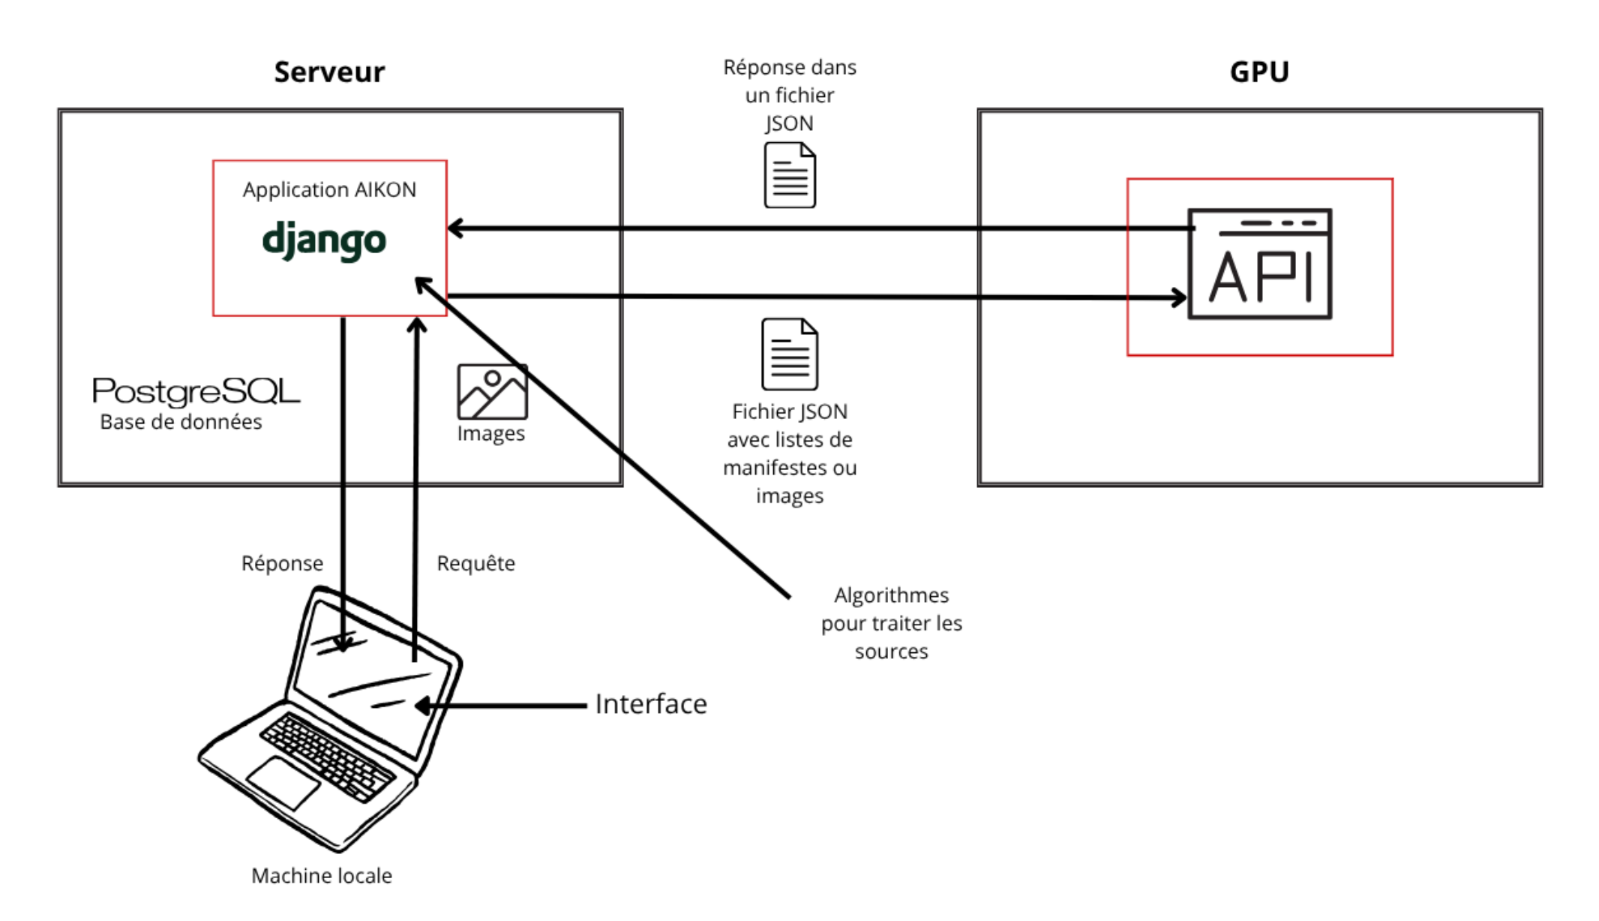
\includegraphics[width=1\textwidth]{images/architecture_aikon.png}
	\caption{Architecture de l'application AIKON}
	\label{fig:architecture_aikon}
\end{figure}

L'utilisateur interagit avec l'application via une interface graphique. Il envoie une requête à l'application qui est hébergée sur un serveur. AIKON est codée en python avec Django. Il s'agit d'un \textit{framework} \textit{open-source} qui permet de développer des applications web robustes facilement. Sur le serveur, il y a également la base de données PostgreSQL et les numérisations du projet. Pour réaliser un traitement automatique des données, l'extraction de \textit{regions} ou la reconnaissance de similarités par exemple, l'application envoie un fichier \gls{json} avec des listes de manifestes ou d'images à l'\gls{api} déployée sur le \gls{gpu}. Lorsqu'elle reçoit le fichier  \gls{json}, elle le traite avec l'algorithme choisi par l'utilisateur via l'interface graphique. Ensuite, l'\gls{api} renvoie un nouveau fichier \gls{json} avec des annotations à l'application. Pour finir, l'utilisateur peut accéder aux résultats de l'opération sur son interface graphique pour les utiliser.

\subsubsection{Le modèle de données}

\gls{aikon} possède un modèle de données commun à tous les projets qui l'exploitent mais il reste extensible pour s'adapter aux besoins spécifiques de ces derniers. Il est composé de plusieurs tables connectées entre elles.

\begin{figure}[H]
	\centering
	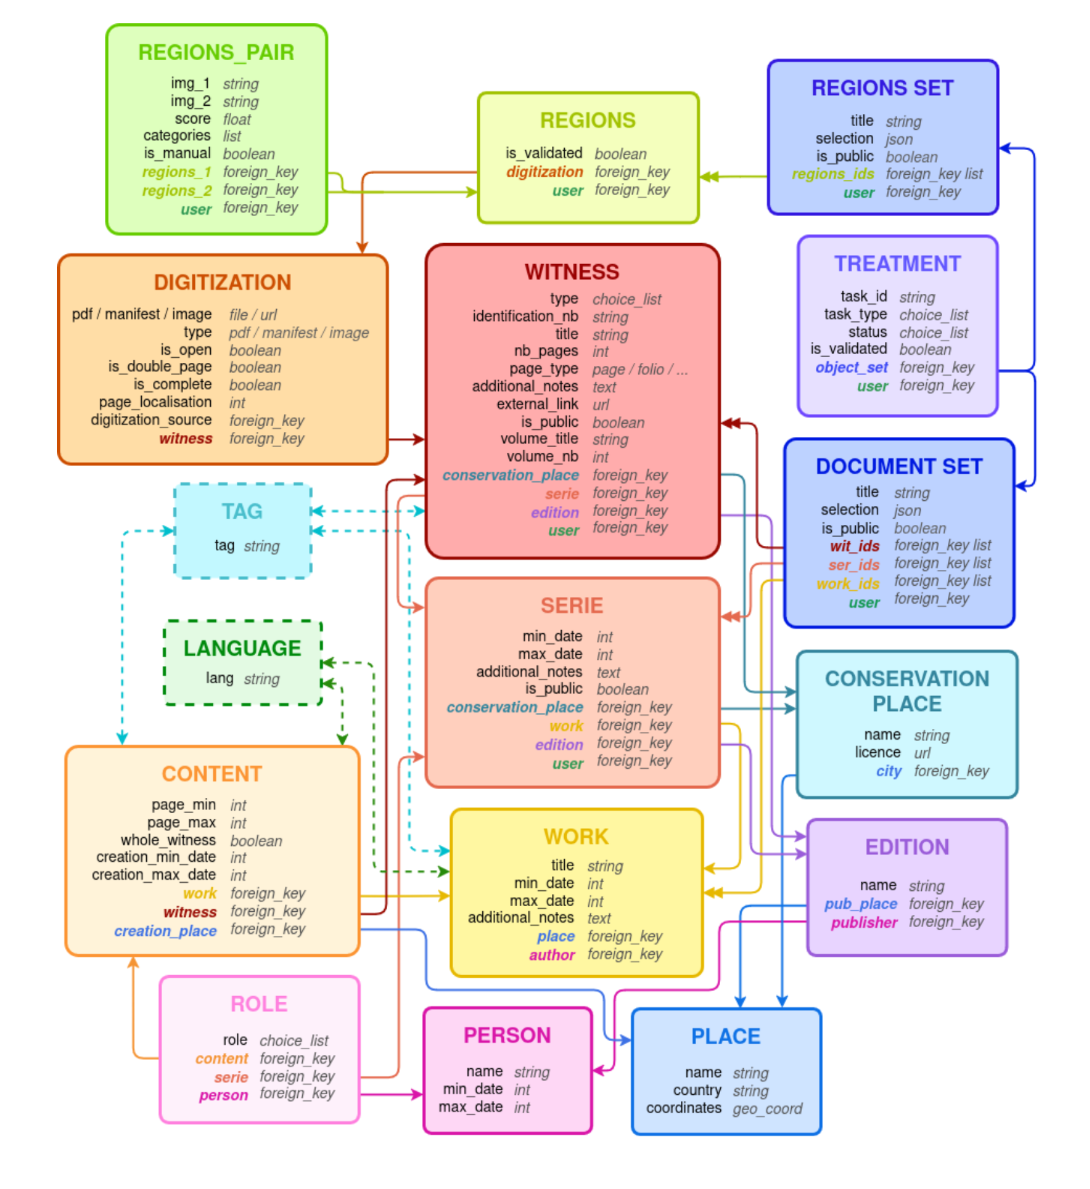
\includegraphics[width=1\textwidth]{images/modele_donnees_aikon.png}
	\caption{Modèle de données de l'application AIKON}
	\label{fig:modele_donnees}
\end{figure}

La table centrale du modèle de données est \textit{witness}. Elle contient toutes les informations relatives à chaque document numérisé mis en ligne sur l'application. Elle est reliée aux autres tables par le biais de \textit{foreign keys}. 

Dans ce modèle de données, nous retrouvons des tables reliées à des fonctions différentes : 
\begin{itemize}
	\item La description du \textit{witness} et de ses métadonnées : \textit{witness, conservation place, edition, place, person, role, content, language}
	\item La numérisation du \textit{witness} : \textit{digitization}
	\item L'organisation des \textit{witnesses} en sous-séries : \textit{serie, works}. Les \textit{series} sont des groupes de \textit{witnesses} partageant une cohérence commune comme un volume d'édition ou des fragments de manuscrits conservés dans différentes institutions. Les \textit{works} sont des productions intellectuelles abstraites qui englobent ses idées fondamentales et son contenus. 
	\item : Les traitements automatiques : \textit{treatment, regions set, regions, region pairs} 
\end{itemize}

Cependant, certaines tables ont plusieurs fonctions grâce aux liens qui les relient entre elles. 

Dans le cadre de notre étude, nous allons surtout nous concentrer sur les tables relatives au traitement automatique des sources et notamment à \textit{region pairs}. \\

L'application AIKON est née des projets \gls{eida} et \gls{vhs}. Il existe également une instance \textit{demo} utilisée par l'Ecole nationale des ponts et chaussées.
D'autres projets souhaiteraient utiliser AIKON à l'avenir pour traiter leurs sources. C'est le cas du projet \textit{High Vision} dont le but est d'étudier en s'aidant de la \textit{computer vision} des photographies de presse datant de la fin XIXe siècle au début du XXe siècle qui ont été numérisées en masse\footcite{HIGHVISIONProjet2025}.


\subsection{Le projet VHS}

\gls{vhs} est un projet qui a pour but de mettre en place une nouvelle approche de l'étude historiques du savoir scientifique en utilisant les outils numériques pour l'analyse d'image\footcite{Presentation}.Il a permis de constituer un nouveau \textit{dataset} d'illustrations scientifiques du Moyen-Age et de l'époque moderne. Cela a permis d'extraire près de 235000 images à partir de 405000 pages du corpus. Suite à l'annotation manuelle des résultats d'extraction d'image, 8000 d'entre-elles ont été validées par des historiens\footcite{fouadComputerVisionHistorical2023}. Ce \textit{dataset} est composé de quatre corpus sélectionnés pour leur diversité en ce qui concerne leur thématique, leur époque et leur aire géographique. 
Nous avons d'abord le \textit{Physiologus} un texte rédigé vers le IIe siècle de notre ère à Alexandrie. Il est composé d'une centaine de manuscrits écrits en grec dont 13 d'entre eux sont illustrés. Ces derniers ont été réalisés entre le XIe et le XVIe siècle et ils ont été diffusés dans tout l'Occident chrétien. Nous avons pu extraire environ 680 images d'animaux, de plantes et de minéraux. 
Le deuxième corpus concerne le \textit{De materia medica} écrit vers 77 de notre ère par Dioscoride. Il est conservé dans 65 manuscrits grecs. 17 d'entre eux réalisées entre le VIe et le XVIe siècle sont illustrés d'environ 8340 images de plantes, d'animaux et de minéraux. 
Les deux derniers corpus contiennent des planches de \textit{l'Encyclopédie} de Diderot et d'Alembert publiées entre 1751 et 1772 mais aussi leurs sources et leur inclusion ultérieure dans d'autres encyclopédies. Les deux thèmes principaux de ces corpus sont l'histoire naturelle et les sciences mathématiques. 
Ainsi, nous retrouvons au sein du projet \gls{vhs} à la fois deux œuvres datant de l'Antiquité et ayant été diffusés durant tout le Moyen Age et l'époque moderne\footcite{Corpus}.



\subsection{Le projet EIDA}

\gls{eida} est un projet d'envergure internationale qui a pour but l'étude et l'analyse des diagrammes de tradition ptolémaïque dans un corpus de témoins allant du IXe siècle au XIXe siècle avec des sources en latin, hébreu, sanskrit, byzantin, perse, grec, chinois et arabe. Il rassemble deux équipes de recherche. Le laboratoire \gls{lte} de l'Observatoire de Paris s'occupe principalement de la partie histoire des sciences du projet tandis que l'équipe IMAGINE de l'Ecole nationale des Ponts et Chaussées gère la partie \textit{computer vision}\footcite{albouyAIKONComputerVision}. 

Le but du projet serait de développer des outils pour que les chercheurs puissent explorer, visualiser le corpus, communiquer les résultats lors de conférences et réaliser des éditions de diagrammes nativement numériques \footcite{Conference2023EIDA2023}.

Le projet encore en cours s'est déroulé en plusieurs étapes. La première concernait la constitution du corpus. Les chercheurs cherchent à étudier le diagramme sous un angle documentaire en tant que artefact et sous son angle épistémique en tant qu'outil de compréhension pour les acteurs historiques\footcite{Conference2023EIDA2023}.

Suite au développement des premiers outils numériques de la plateforme, il a été possible d'appliquer aux sources de premiers traitements automatiques. L'extraction puis la reconnaissance automatique de \textit{region pairs} et le calcul de similarité ont permis de distinguer les diagrammes en double et de les interpréter dans plusieurs traditions, œuvres et témoins\footcite{Conference2024Graphic2024}.

Les chercheurs ont pu réaliser de premières observations. Il se trouve que les diagrammes peuvent être regroupés en fonction de leurs similarités. Un diagramme peut être rattaché à une œuvre, à une thématique ou à une famille\footcite{Conference2025Long2025}. 

Les chercheurs se réunissent régulièrement pour mener une réflexion autour du projet lors de conférences et séminaires. 
 

Sur le long terme, le but du projet serait de mettre à disposition des chercheurs une interface utilisateur sur le modèle de celle de \gls{dishas}, un projet antérieur mené par l'Observatoire de Paris. \\





 